\documentclass[slidestop,mathserif,8pt]{beamer}
\usetheme{Warsaw} % Beamer theme v 3.0

\usepackage{graphicx,pgfarrows,pgfnodes,psfrag}
\usepackage{amssymb,amsmath,wasysym	}
%\usepackage[]{color}
\usepackage{epstopdf}

\newtheorem{thm}{Theorem}[section]
\newtheorem{ex}{Example}
\newtheorem{cor}{Corollary}[section]
\newtheorem{prop}[thm]{Proposition}
\newtheorem{lem}[thm]{Lemma}
\newtheorem{conjec}[thm]{Conjecture}
\theoremstyle{remark}
\newtheorem*{rem}{Remark}
\theoremstyle{definition}
\newtheorem{defn}{Definition}[section]
\theoremstyle{assumption}
\newtheorem{ass}{Assumption}[section]


\newtheorem{assumption}{Assumption}
\newtheorem{algoritmo}{Algorithm}
\newtheorem{proposition}{Proposition}

\newcommand{\norm}[1]{\left\Vert#1\right\Vert}
\newcommand{\norminf}[1]{\left\Vert#1\right\Vert_{\infty}}
\newcommand{\abs}[1]{\left\vert#1\right\vert}
\newcommand{\dz}{\textnormal{dz}}
\newcommand{\sat}{\textnormal{sat}}
\newcommand{\sign}{\textnormal{sign}}
\newcommand{\diag}{\textnormal{diag}}
\newcommand{\blockdiag}{\textnormal{blockdiag}}
\newcommand{\rank}{\textnormal{rank}}
\newcommand{\fracpar}[2]{\frac{\partial #1}{\partial #2}}
\newcommand{\diff}[2]{\frac{\partial #1}{\partial #2}}

\newcommand{\sube}[2]{\begin{subequations}\label{#1}
\begin{align} #2\end{align}\end{subequations}}

\def\bbm#1\ebm{\begin{bmatrix}#1\end{bmatrix}} %Puo' servire racchiudere l'argomento fra graffe
%\def\hinf{\mathcal{H}_\infty}
%\def\rhinf{\mathcal{RH}_\infty}
\newcommand {\Qend}{~\hfill$\blacksquare$}

\newcommand{\qend}{~\hfill$\square$\vspace{0.5mm}}
\def\ie{{\it i.e.~}}
\def\eg{{\it e.g.~}}
\newcommand{\R}{\mathbb{R}}
\newcommand{\N}{\mathbb{R}}
\def\usigma{\underline{\sigma}}
\def\legendsize{\tiny}

\usepackage{hyperref}
\newenvironment{figura}[3]
    {
    \begin{figure}[H]
    { \normalsize\begin{center}
    \resizebox{#2\columnwidth}{!}{\includegraphics{figs/#1}}
    \end{center}}
    \caption{#3}
    }
    {
    \end{figure}
    \noindent
    }
\newcommand{\fig}[3]{\begin{figura}{#1}{#2}{#3} \label{#1} \end{figura}}
\newcommand{\figsizerate}{0.7}
\setbeamertemplate{footline}[page number]

%\definecolor {white}    {rgb}     {1} % {1,   1,   1}
%\definecolor {black}     {rgb}    {0} 
%\definecolor {gray}       {rgb}   {.9}
\definecolor {red} {rgb} {1,   0,   0}
\definecolor {green}{rgb}         {0,   1,   0}
\definecolor {blue}{rgb}    {0,   0,   1}
\definecolor {cyan}{rgb} {0,   1,   1}
\definecolor {magenta}      {rgb} {1,   0,   1}
\definecolor {yellow}  {rgb}      {1,   1,   0}
\definecolor {darkred}   {rgb}    {.8,  0,   0}
\definecolor {middlered} {rgb}    {.9,  0,   0}
\definecolor {lightred}  {rgb}    {1,   0,   0}
\definecolor {darkgreen}  {rgb}{0 ,  .6,  0}
\definecolor {middlegreen}  {rgb} {0,   .8,  0}
\definecolor {lightgreen}  {rgb}  {0,   1,   0}
\definecolor {darkblue}  {rgb}    {0,   0,   .8}
\definecolor {middleblue}  {rgb}  {0,   0,   .9}
\definecolor {lightblue}  {rgb}   {0,   0,   1}
\definecolor {darkcyan}    {rgb}  {.6,  .8,  .8}
\definecolor {middlecyan}  {rgb}  {0,   .8,  .8}
\definecolor {darkmagenta}  {rgb} {.8,  .6,  .8}
\definecolor {middlemagenta} {rgb}{1,   0,   .6}
\definecolor {darkyellow} {rgb}   {.8,  .8,  .6}
\definecolor {middleyellow} {rgb} {1,   1,   .2}
%\definecolor {darkgray}  {rgb}    {.5}
%\definecolor {middlegray}  {rgb}  {.7}
%\definecolor {lightgray}  {rgb}   {.9}
\definecolor{Dblue}{rgb}{.255,.41,.884}



\def\labelsize{\small}
\def\colorize<#1>{%
\temporal<#1>{\color{red!50}}{\color{black}}{\color{black!50}}}
\newcommand{\redt}[1]{{\color{red} #1}}
\newcommand{\greent}[1]{{\color{darkgreen} #1}}
\newcommand{\bluet}[1]{{\color{blue} #1}}

\vspace{-0.5cm}
\title[Runaway Modeling] {Plasma elongation of RE beam}
%\author{\vspace{6pt}{\small 
%Daniele Carnevale } 
%\vspace{30pt}\newline
%{\small  Dipartimento di Ing. Civile ed Ing. Informatica (DICII),
%\newline University of Rome ``Tor Vergata''\\}\vspace{0.4cm}
%{\footnotesize \underline{References:} \\[3mm]
%- K. B. Ariur and M. Krsti\`c. ``Real-Time Optimization by 
%Extremum-Seeking Control '', John Wiley \& Sons, 2003\\
%}
%} 

%\date{\small 29 January 2014\\
%}

 
\begin{document}

\frame{\titlepage
\vspace{-0.5cm}
}

\section[Model 1 ]{Model 1}
%\subsection[Static Map ]{Static Map}

\frame{\frametitle{Plasma elongation}
\small

The plasma elongation k is proportional to 

\begin{align}
	k = \frac{b}{a} \propto \frac{I_F}{I_P}
\end{align}

where $I_F$ is the current of active coil F and $I_P$ is the plasma current.\\

Esiste una correlazone tra il coefficiente k e la perdita del plasma nella fasa di plateau?\\

Analisi degli spari: 38864, 38865, 38869, 38513, 38519

}

\frame{\frametitle{Plasma elongation. Shots 35965, 36569, 36574 and 36634}
	\small
	
	\begin{figure}
		\centering
		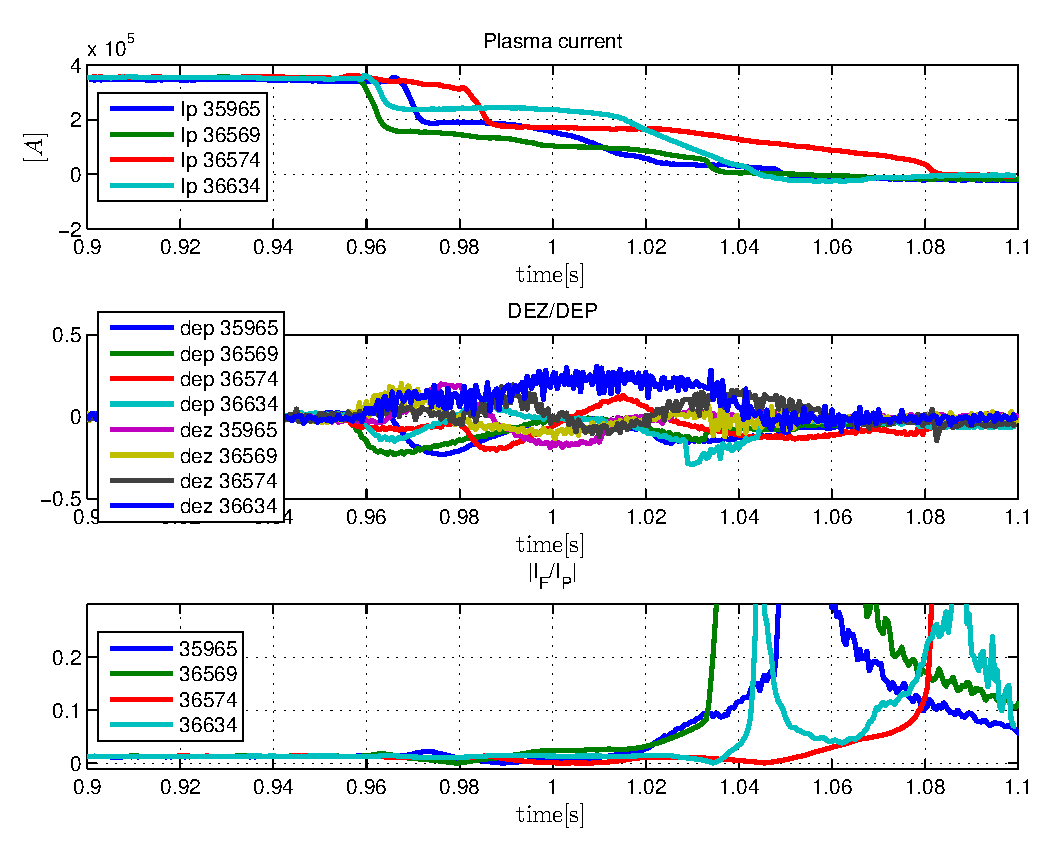
\includegraphics[width=1\linewidth]{figs/b.eps}
		\caption[Shots 38864, 38865 and 38869]{Shots 38864, 38865 and 3886}
		\label{fig:correlazioneIfIp3581335819}
	\end{figure}

}

\frame{\frametitle{38513, 38519}
	\small 
	\vspace{-4mm}
	\begin{figure}
		\centering
		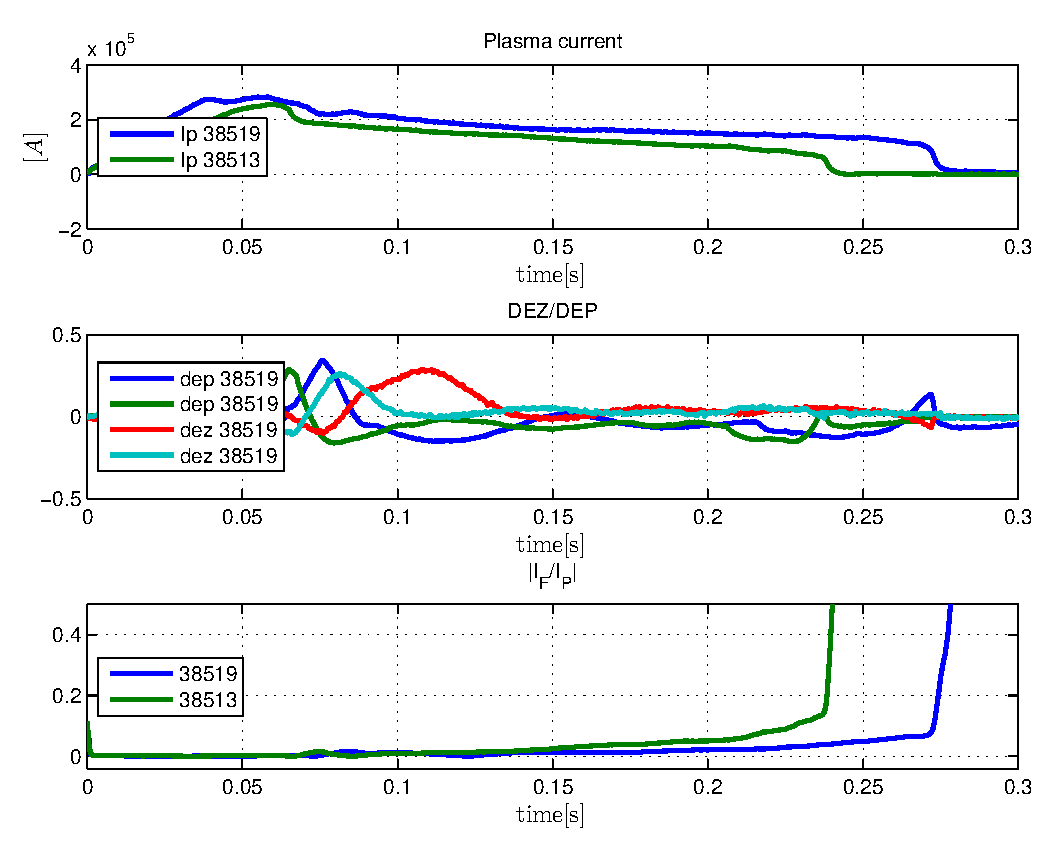
\includegraphics[width=1\linewidth]{figs/c.eps}
		\caption[Shot 38513 and 38519]{Shot 38513 and 38519}
		\label{fig:correlazioneIfIp3581335819}
	\end{figure}		
}


\frame{\frametitle{38864, 38865 and 38869}
\small 
\begin{figure}
\centering
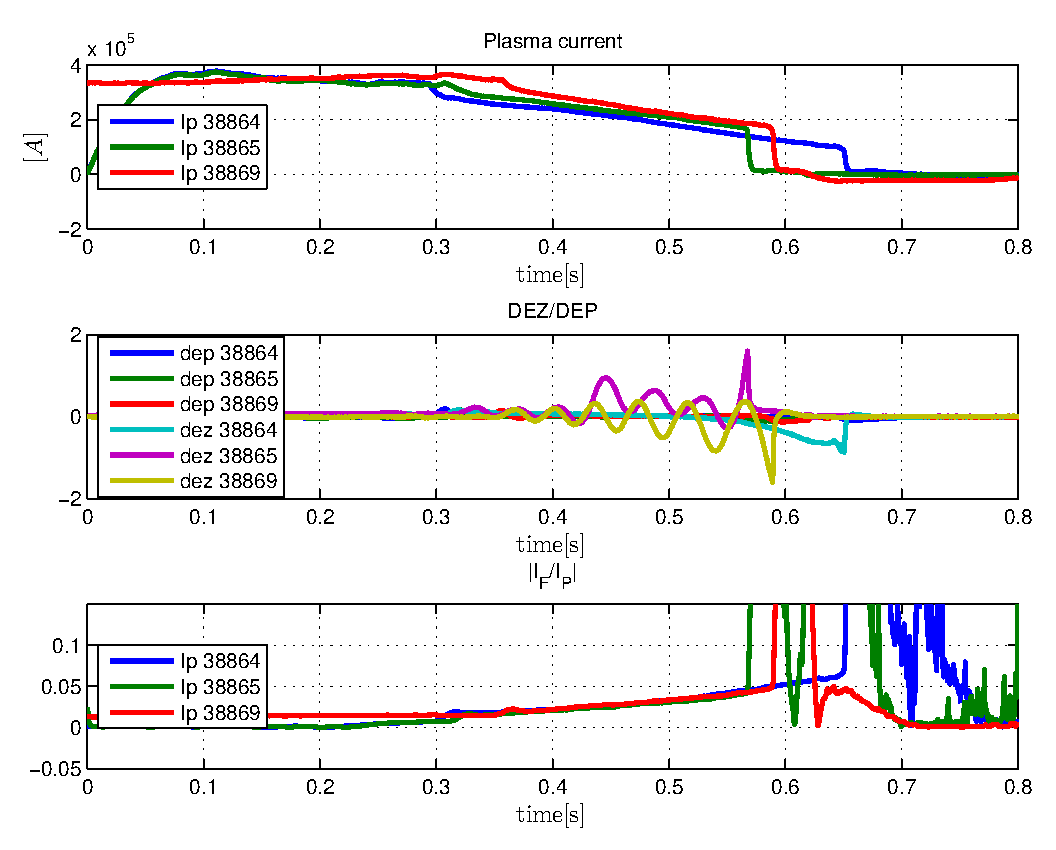
\includegraphics[width=1\linewidth]{figs/a.eps}
\caption[Shots 38864, 38865 and 38869]{Shots 38864, 38865 and 3886}
\label{fig:correlazioneIfIp3581335819}
\end{figure}


}








%\bibliographystyle{siam} 
%\bibliography{ModeRunaway_v5}

\end{document}




